\documentclass[11pt]{article}
\usepackage[a4paper,margin=2.4cm]{geometry}
\usepackage{lmodern}
\usepackage[T1]{fontenc}
\usepackage{microtype}
\usepackage{graphicx}
\usepackage{booktabs}
\usepackage{tikz}
\usetikzlibrary{arrows.meta,positioning,shapes.geometric}
\usepackage{pgfplots}
\pgfplotsset{compat=1.17}
\usepackage[hidelinks]{hyperref}
\hypersetup{
  pdftitle={ResearchPDF: A Paper-First PDF Viewer for Chrome},
  pdfauthor={ResearchPDF},
  pdfsubject={A guided tour of ResearchPDF, opened by its welcome page},
  pdfkeywords={PDF viewer, papers, annotations, Google Drive sync}
}

\title{\textbf{ResearchPDF: A Paper-First PDF Viewer for Chrome}}
\author{The ResearchPDF tour\\[2pt]\small\url{https://research-pdf.croksuter.com}}
\date{}

\begin{document}
\maketitle

\begin{abstract}
\noindent
You are reading this document inside ResearchPDF. It is a short paper about
the extension itself, so that every feature it describes can be tried right
here: the tab you are in, the paper bar above, the annotation tools, and the
figure capture. Each section ends with a \emph{Try it} line.
\end{abstract}

\section{One tab for your papers}
PDFs opened from the web or from your computer gather in one \emph{PDF tab},
with a tab strip of its own, instead of scattering among your web tabs.
Papers go into \emph{projects}: every new PDF starts in the default project,
and \emph{Move to project} sends it elsewhere. Projects can be grouped in
folders, ordered by dragging, and given an icon, an emoji or a color---which
also becomes the icon of their tab in Chrome. Closing a project's tab and
opening it later brings back the same papers.

\smallskip\noindent\emph{Try it:} press \textsf{Alt+Shift+\(\rightarrow\)} to
move to the next tab, \textsf{Alt+W} to close one and
\textsf{Alt+Shift+T} to bring it back. The house button opens \emph{Home}:
everything you have opened, with reading progress, filters and search.

\section{Knowing the paper}
When a document is recognised as a paper---by its DOI, its arXiv identifier
or its title---a bar under the toolbar shows its venue and year, its
citations (with a per-year chart), its references, and BibTeX or APA ready to
copy. The data comes from open scholarly databases
(Table~\ref{tab:sources}); only identifiers are sent to them.

\begin{table}[h]
\centering
\caption{Where the paper bar gets its data.}
\label{tab:sources}
\begin{tabular}{@{}lll@{}}
\toprule
Source & Provides & Reference \\
\midrule
OpenAlex & venues, yearly citations, references & \cite{openalex} \\
Crossref & DOIs, publishers, reference counts & \cite{crossref} \\
Semantic Scholar & merged preprint and published counts & \cite{s2} \\
arXiv & preprints and their versions & --- \\
\bottomrule
\end{tabular}
\end{table}

\noindent\emph{Try it:} open any paper from arXiv or a publisher; this tour
itself is not a published paper, so its bar says so.

\section{Notes that travel}
Highlights, pen strokes and text notes are kept per document, and a document
is recognised by its content rather than its file name. Connect a Google
account and they follow you---with the page you were on---to every Chrome
profile and device, through a hidden app-only folder in \emph{your own}
Drive (Figure~\ref{fig:sync}). The PDF files themselves are never uploaded.

\begin{figure}[h]
\centering
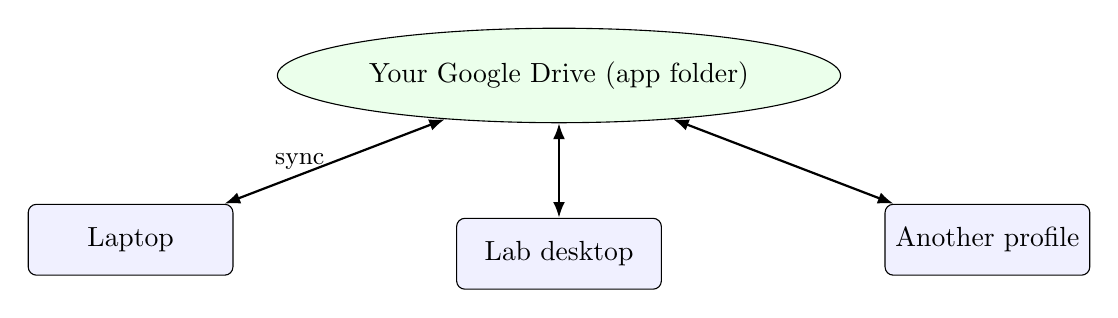
\begin{tikzpicture}[
  node distance=1.2cm and 1.6cm,
  dev/.style={draw, rounded corners=3pt, minimum width=2.6cm, minimum height=0.9cm, fill=blue!6},
  cloud/.style={draw, ellipse, minimum width=3.6cm, minimum height=1.2cm, fill=green!8},
  link/.style={{Latex[length=2mm]}-{Latex[length=2mm]}, thick}
]
\node[cloud] (drive) {Your Google Drive (app folder)};
\node[dev, below left=of drive] (lap) {Laptop};
\node[dev, below=of drive] (lab) {Lab desktop};
\node[dev, below right=of drive] (pro) {Another profile};
\draw[link] (lap) -- node[left, font=\small] {sync} (drive);
\draw[link] (lab) -- (drive);
\draw[link] (pro) -- (drive);
\end{tikzpicture}
\caption{Annotations and reading positions sync through an app-only folder in
your own Drive; no server of ours is involved.}
\label{fig:sync}
\end{figure}

\noindent\emph{Try it:} open the annotation tools (the pen button), highlight
a sentence of this paragraph, and reopen this document on another device.

\section{Figures in one key}
Press \textsf{S} and drag over any region to copy it as an image, with its
source. Press \textsf{S} again and the figures and tables of the page are
found for you---by a small layout model running on your device
\cite{ppdoclayout} together with the PDF's own captions. Click one to copy it.
Figure~\ref{fig:plot} and Table~\ref{tab:sources} are good targets.

\begin{figure}[h]
\centering
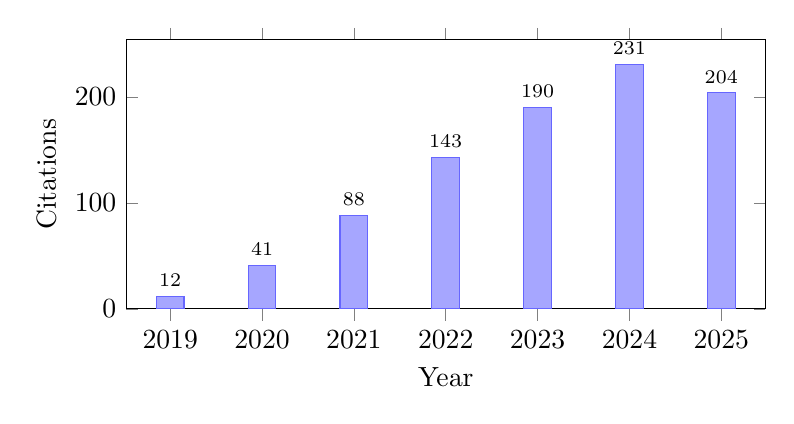
\begin{tikzpicture}
\begin{axis}[
  ybar, bar width=10pt, width=0.8\linewidth, height=5cm,
  xlabel={Year}, ylabel={Citations},
  symbolic x coords={2019,2020,2021,2022,2023,2024,2025},
  xtick=data, ymin=0, enlarge x limits=0.08,
  nodes near coords, every node near coord/.append style={font=\scriptsize}
]
\addplot[fill=blue!35, draw=blue!60] coordinates {(2019,12) (2020,41) (2021,88) (2022,143) (2023,190) (2024,231) (2025,204)};
\end{axis}
\end{tikzpicture}
\caption{An example of the per-year citation chart the paper bar draws
(illustrative numbers).}
\label{fig:plot}
\end{figure}

\noindent\emph{Try it:} press \textsf{S} twice now, then click a figure.

\begin{thebibliography}{9}
\bibitem{openalex} J.~Priem, H.~Piwowar, and R.~Orr. OpenAlex: A fully-open
index of scholarly works, authors, venues, institutions, and concepts.
\emph{arXiv:2205.01833}, 2022.
\bibitem{crossref} G.~Hendricks, D.~Tkaczyk, J.~Lin, and P.~Feeney. Crossref:
The sustainable source of community-owned scholarly metadata.
\emph{Quantitative Science Studies}, 1(1):414--427, 2020.
\bibitem{s2} R.~Kinney et al. The Semantic Scholar Open Data Platform.
\emph{arXiv:2301.10140}, 2023.
\bibitem{ppdoclayout} T.~Sun et al. PP-DocLayout: A unified document layout
detection model to accelerate large-scale data construction.
\emph{arXiv:2503.17213}, 2025.
\end{thebibliography}

\end{document}
